\chapter{QPCC Solver}
\label{chapter:AppendixA}

\section{QPCC for Contact}

The QPCC problem for contact modeling is:

\begin{align}
\label{eqn:optimization}
 \min_{\dot{\vc{p}}^{n+1}, \vc{u},\vc{f}_\perp,\vc{f}_\parallel,\lambda}& G(\dot{\vc{p}}^{n+1}, \vc{u})  \\
\nonumber  \mathrm{subject\;} \mathrm{to} &\\
\nonumber &\vc{u}_{lb} \leq \vc{u} \leq \vc{u}_{ub}\\
\label{eqn:dynamicConstraint} &\widetilde{\vc{M}}\dot{\vc{p}}^{n+1} = \vc{f}_c + \vc{A}\vc{u} + \widetilde{\vc{f}}^n\\
\label{eqn:contactConstraint} &\vc{0} \leq \left[ \begin{array}{c} \vc{f}_\perp \\ \vc{f}_\parallel \\ \lambda \end{array} \right] \perp
 \left[ \begin{array}{c} \vc{N}^T\dot{\vc{p}}^{n+1} \\ \vc{D}^T \dot{\vc{p}}^{n+1} + \vc{E} \lambda \\ \mu \vc{f}_\perp - \vc{E}^T \vc{f}_\parallel \end{array} \right] \geq \vc{0}
\end{align}
where $G(\dot{\vc{p}}^{n+1}, \vc{u})$ is a convex quadratic objective function of next velocities $\dot{\vc{p}}^{n+1}$ and control variables $\vc{u}$, which are bounded by $\vc{u}_{lb}$ and $\vc{u}_{ub}$.

Equation \ref{eqn:dynamicConstraint} is the discretized dynamic equation (Equation 8 in the paper), where $\widetilde{\vc{M}}$ is the mass matrix with terms from implicit integrator, $\vc{f}_c$ and $\vc{Au}$ are the contact force and control force (scaled by the time step) respectively, and $\widetilde{\vc{f}}^n$ accounts for all other terms in the dynamic equation.

Equation \ref{eqn:contactConstraint} is the LCP formulation to regulate contact velocity and contact force, $\vc{f}_c=\vc{N}f_{\perp}+\vc{Df}_{\parallel}$, where $\vc{N}$ is the unit normal vector, $\vc{D}$ is a set of tangential directions at the contact point, and $f_{\perp}$ and $\vc{f}_{\parallel}$ are the magnitudes of normal and tangent forces. $\mu$ is the friction coefficient and $\lambda$ is an auxiliary variable whose physical meaning is related to the tangent velocity of a sliding contact. This form is slightly more general than the QPCC formulation (Equation 11) in the paper.

\section{Implementation of QPCC Solver for Contact}

\begin{algorithm}[ht]
($\vc{x}^*$, $f^*$) = Solve(QPCC)\\
\Begin
{
    ithIter = 0\;
    $f^* \leftarrow \infty$\;
    $\vc{x}^* \leftarrow$ null\;
    priority\_queue $\leftarrow$ []\;
    visitedQP\_set $\leftarrow$ \{\}\;
    CCSpec $\leftarrow$ GenerateInitialGuess()\;
    QP $\leftarrow$ GenerateQP(QPCC, CCSpec)\;
    (QP.minimizer, QP.fval) $\leftarrow$ QP.Solve()\;
    priority\_queue.Enqueue(QP)\;

    \While{visitedQP\_set.Size() $<$ maxNumVisitedQP and priority\_queue.Empty() $=$ False}
    {
        QP $\leftarrow$ priority\_queue.Dequeue()\;
        visitedQP\_set.Add(QP)\;
        \If{QP.fval $< f^*$}
        {
            $f^* \leftarrow$ QP.fval\;
            $\vc{x}^* \leftarrow$ QP.minimizer\;
        }
        childQP\_list $\leftarrow$ GenerateChildQP(QPCC, QP, CCSpec)\;

        \ForEach{childQP in childQP\_list}
        {
            \If{visitedQP\_set.Find(childQP)}
            {
                continue\;
            }
            (childQP.minimizer, childQP.fval) $\leftarrow$ childQP.Solve()\;
            priority\_queue.Enqueue(childQP)\;
        }
        ithIter $\leftarrow$ ithIter + 1\;
    }
    \Return{($\vc{x}^*$, $f^*$)}\;
}
\caption{Pseudo-code of the QPCC solver.} \label{alg:main}
\end{algorithm}


Algorithm \ref{alg:main} summarizes the implementation of our QPCC solver. The solver takes the QPCC (Equation \ref{eqn:optimization}-\ref{eqn:contactConstraint}) as input and outputs the minimizer $\vc{x}^*$ and minimum objective function value $f^*$. Our iterative QPCC solver starts with an initial guess of the contact situation, which is a set of linear constraints that are compatible with the complementarity conditions. Function \emph{GenerateInitialGuess} in Line 8 generates such an initial guess. We usually choose static contact situation as the initial guess:
\begin{align}
\nonumber & \vc{0} \leq \vc{f}_\perp, & \vc{N}^T\dot{\vc{p}}^{n+1} = \vc{0}\\
\nonumber & \vc{0} \leq \vc{f}_\parallel, &  \vc{D}^T \dot{\vc{p}}^{n+1} + \vc{E} \lambda = \vc{0}\\
\nonumber & \vc{0} = \lambda, & \mu \vc{f}_\perp - \vc{E}^T \vc{f}_\parallel \geq \vc{0} \\
 \nonumber
\end{align}
Occasionally, this initial guess is inconsistent with the dynamic constraints (Equation \ref{eqn:dynamicConstraint}), resulting in an infeasible problem. In
such a case, we solve the Mixed LCP problem (Equation \ref{eqn:dynamicConstraint} and \ref{eqn:contactConstraint}), assuming $\vc{u}=\vc{0}$, to obtain a feasible initial guess. The output of \emph{GenerateInitialGuess} is a boolean array \emph{CCSpec} that specifies a set of linear constraints from the complementarity conditions. If the $i$th entry of \emph{CCSpec} is True, we choose the linear constraints $Cond_1 = 0$ and $Cond_2 \geq 0$ for the $i$th pair of complementarity conditions $0\leq Cond_1 \perp Cond_2 \geq 0$. If it is False, we choose $Cond_1 \geq 0$ and $Cond_2 = 0$.

Function \emph{GenerateQP} in Line 9 generates a QP by replacing the complementarity conditions of QPCC with the linear constraints specified in \emph{CCSpec}.
In Line 10, we solve the initial QP and record its minimizer and minimal function value. We add this QP to an priority queue, which sorts the QP's by their function values in an increasing order. Line 12 starts the iteration, which terminates until the number of explored QP's exceeds a threshold or the priority queue is empty.

In each iteration, we retrieve the QP at the head of the queue (Line 13), add it to the set of explored QP's and update $f^*$ and $\vc{x}^*$ if necessary (Line 14-17). Function \emph{GenerateChildQP} generates a list of new QP's by pivoting complementarity conditions (Line 18), which we will discuss
in the next paragraph. For each new QP in the list, if it has been already explored, we discard it (Line 20-21). Otherwise, we solve the new QP and add it to the queue (Line 22-23). When the algorithm terminates, we output the best minimizer and function value that we found during the iterations (Line 25).

\begin{algorithm}[!b]
QP\_list = GenerateChildQP(QPCC, QP, CCSpec)\\
\Begin
{
    \ForEach{ i in Contacts.Size()}
    {
        ($\dot{\vc{p}}$, $f_{\perp}^{i}$, $\vc{f}_{\parallel}^{i}$, $\lambda^{i}$) $\leftarrow$ ExtractFromMinimizer(QP.minimizer)\;
        newCCSpec $\leftarrow$ CCSpec\;
        id $\leftarrow$ IdInCC($0 \leq f_{\perp}^{i} \perp (\vc{N}^{i})^T\dot{\vc{p}} \geq 0$)\;
        \If{CCSpec[id] $=$ True and $(\vc{N}^{i})^T\dot{\vc{p}} $=$ 0$}
        {
            newCCSpec[id] $\leftarrow$ False\;
            newQP $\leftarrow$ GenerateQP(QPCC, newCCSpec)\;
            QP\_list.Add(newQP)\;
        }
        \ElseIf{CCSpec[id] $=$ False and $f_{\perp}^i $=$ 0$}
        {
            newCCSpec[id] $\leftarrow$ True\;
            newQP $\leftarrow$ GenerateQP(QPCC, newCCSpec)\;
            QP\_list.Add(newQP)\;
        }


        id $\leftarrow$ IdInCC($0 \leq \lambda_{\perp}^{i} \perp \mu f_{\perp}^i-(\vc{E}^{i})^T\vc{f}_{\parallel}^i \geq 0$)\;
        id\_list $\leftarrow$ IdInCC($\vc{0}\leq\vc{f}_{\parallel}^i\perp (\vc{D}^i)^T\dot{\vc{p}}+\vc{E}^i\lambda^i \geq \vc{0}$)\;

        \If{CCSpec[id] $=$ True and $\mu f_{\perp}^i-(\vc{E}^{i})^T\vc{f}_{\parallel}^i = 0$}
        {
            newCCSpec[id] $=$ False\;
            \ForEach{id1 in id\_list}
            {
                newCCSpec[id1] $\leftarrow$ True\;
            }
            $\vc{f} \leftarrow \vc{D}^i \vc{f}_{\parallel}^i$\;
            j $\leftarrow \argmax_{k} \vc{f}^T (\vc{D}^i$.Col(k)$)$\;
            newCCSpec[j] $\leftarrow$ False\;
            newQP $\leftarrow$ GenerateQP(QPCC, newCCSpec)\;
            QP\_list.Add(newQP)\;
        }
        \ElseIf{CCSpec[id] $=$ False and $\lambda^i = 0$}
        {
            newCCSpec[id] $\leftarrow$ True\;
            \ForEach{id1 in id\_list}
            {
                newCCSpec[id1] $\leftarrow$ False\;
            }
            newQP $\leftarrow$ GenerateQP(QPCC, newCCSpec)\;
            QP\_list.Add(newQP)\;
        }

    }
    \Return{QP\_list}\;
}

\caption{Generate a list of new QP's based on the minimizer of the current QP} \label{alg:childQP}
\end{algorithm}

We summarize the detail of \emph{GenerateChildQP} in Algorithm \ref{alg:childQP}. The input of \emph{GenerateChildQP} includes QPCC, current QP and its constraint specification for complementarity conditions: \emph{CCSpec}. In Line 4, we extract the solution for each contact from the minimizer of the QP. Function \emph{ExtractFromMinimizer} selects the correct components associated with a specific contact point from the minimizer. In Line 6, we identify the index of the normal force-velocity condition pair for the $i$th contact, where \emph{IdInCC} returns the index of a specific pair among all complementarity conditions. Line 7 identifies the case of contact establishment and performs the corresponding pivoting (Line 8). Line 11 checks whether the contact is about to break and pivots the constraint accordingly, which enables the contact breakage (Line 12). Line 15-16 identify the indices of friction cone and friction direction conditions associated with the $i$th contact. If the static friction force has reached the boundary of friction cone, we switch the contact situation from static to sliding (Line 17-18) and estimate the sliding friction direction using the static friction direction (Line 19-23). We apply the opposite pivoting (from sliding to static) when the
sliding velocity reaches zero (Line 26-29). A new QP is generated under the new contact situation and added into the list of new QP's (Line 9-10, 13-14, 24-25 and 30-31) whenever pivoting happens. After processing through all the contact points, the function returns the new QP list.

\section{Test Case}
It is nontrivial to test and debug an implementation of a QPCC solver. We propose the following test case problem: A particle with mass $m$ lies on the ground and it wants to jump up. The particle can only control a jumping force $f\vc{N}$, where $\vc{N}=(0, 1, 0)$ is the up direction. The magnitude of the jumping force is bounded by $0\leq f\leq f_{ub}$. What is the optimal jumping force if the goal is to jump as high as possible? The answer is trivially using maximal force possible. However, the solution is not necessarily $f_{ub}$ under some contact configuration. Our hope is that the QPCC solver can find the optimal contact configuration such that the optimal solution reaches $f_{ub}$.

One formulation of the above problem is:
\begin{align}
\label{eqn:testCase}
\nonumber \min_{\dot{\vc{p}}, f,f_\perp,\vc{f}_\parallel,\lambda}& -f^2  \\
\nonumber  \mathrm{subject\;} \mathrm{to} &\\
\nonumber &0 \leq f \leq f_{ub}\\
\nonumber &m\dot{\vc{p}} = \Delta t(m\vc{g}+\vc{N}f_{\perp}+\vc{Df}_{\parallel}+\vc{N}f) \\
\nonumber &\vc{0} \leq \left[ \begin{array}{c} f_\perp \\ \vc{f}_\parallel \\ \lambda \end{array} \right] \perp
 \left[ \begin{array}{c} \vc{N}^T\dot{\vc{p}} \\ \vc{D}^T \dot{\vc{p}} + \vc{E} \lambda \\ \mu f_\perp - \vc{E}^T \vc{f}_\parallel \end{array} \right] \geq \vc{0}
\end{align}
where $\Delta t$ is the time step used in the simulation and $\vc{g}$ is gravity.

It is easy to verify that the minimizer is
\begin{displaymath}
(\dot{\vc{p}},f,f_\perp,\vc{f}_\parallel,\lambda)=(\frac{\Delta t}{m}(m\vc{g}+\vc{N}f_{ub}), f_{ub}, 0, \vc{0}, 0)
\end{displaymath}
and the optimal function value is $-f_{ub}^2$. A correctly implemented QPCC solver based on Algorithm \ref{alg:main} and \ref{alg:childQP} should converge to this optimal solution in two iterations. In the first iteration, an initial QP using static contact situation is generated and solved. The solution should be
\begin{displaymath}
(\dot{\vc{p}},f,f_\perp,\vc{f}_\parallel,\lambda)=(0, |m\vc{g}|, 0, \vc{0}, 0)
\end{displaymath}
The function \emph{GenerateChildQP} will pivot the constraint to switch from static contact to contact breakage and generate a new QP. In the second iteration, the solution of this new QP is exactly the optimal solution of the QPCC problem.

Once the implementation passes this simple test case, more challenging cases should be tested. For example, control a single rigid body, an articulated rigid-body system, or a soft body with the presence of contact.

\chapter{Constraints in ODE}
\label{chapter:AppendixB}
We are going to describe how various constraints are formulated in ODE for completeness of presentation.

\paragraph{Joint constraints} Joints that connect two rigid bodies constrain their relative motions.
The hinge, universal and ball joints impose five, four and three constraints respectively, each of which is a linear equality constraint.
\begin{equation}
\vc{J}_A
\left[\begin{array}{c}
\vc{v}_A \\
\vc{\omega}_A
\end{array}\right]-
\vc{J}_B
\left[\begin{array}{c}
\vc{v}_B \\
\vc{\omega}_B
\end{array}\right]
=0
\label{eq:jointConstraint}
\end{equation}
where $\vc{J}_A$ is a row in the Jacobian matrix that maps the velocities of body $A$ to one component of the linear velocity at the joint position or the angular velocity perpendicular to the joint axes.

\paragraph{Actuator constraints}
An actuator is attached to each joint of the human character to enable it to actively control its joint motion. The actuators generate internal torques to track the desired pose given by the IK solver (See Figure 2 in the paper). The following linear equality constraint should be satisfied for each actuated degree of freedom (DOF).
\begin{equation}
\vc{n}^T(\vc{\omega}_A-\vc{\omega}_B)-\tilde{\dot{q}}=0
\label{eq:actuatorConstraint}
\end{equation}
where $\vc{n}$ is the axis of the actuated DOF. $\tilde{\dot{q}}$ is the desired actuator angular speed, which is the difference between the desired and current DOF value, divided by the time step.

\paragraph{Contact constraints}
ODE uses the standard friction pyramid to model the contact forces between the bicycle and the ground. Let $f_\perp$, $f_{\parallel}^1$ and $f_{\parallel}^2$ be the normal and two tangential components of the contact force $\vc{f}_c$.
\begin{displaymath}
\vc{f}_c = f_\perp\vc{n}+f_{\parallel}^1\vc{t}_1+f_{\parallel}^2\vc{t}_2
\end{displaymath}
where $\vc{n}$ is the ground normal, $\vc{t}_1$ and $\vc{t}_2$ are the two orthogonal tangential bases of the ground.

Along the normal direction, the contact velocity and contact force satisfy the following linear complementarity constraints.
\begin{equation}
v_\perp\geq 0, \; f_\perp \geq 0, \; v_\perp f_\perp =0
\label{eq:normalContactConstraint}
\end{equation}
The normal contact velocity $v_\perp$ can be calculated by multiplying the Jacobian at the contact location with the body velocities and then projected along the normal direction.
\begin{equation}
v_\perp=\vc{n}^T\vc{J}\left[\begin{array}{c}
\vc{v} \\
\vc{\omega}
\end{array}\right]
\label{eq:normalVelocity}
\end{equation}
Along the tangential direction, one of the following friction cone conditions must be satisfied.
\begin{equation}
\begin{array}{ll}
v_{\parallel}^i > 0, & f_{\parallel}^i = -\mu f_\perp\\
v_{\parallel}^i < 0, & f_{\parallel}^i = \mu f_\perp\\
v_{\parallel}^i = 0, & -\mu f_\perp \leq f_{\parallel}^i \leq \mu f_\perp
\end{array}
\label{eq:tangentialContactConstraint}
\end{equation}
where $i\in\{1,2\}$ and $\mu$ is the friction coefficient. The tangential velocities $v_{\parallel}^i$ can be calculated similar to eq.~(\ref{eq:normalVelocity}).

The dynamics equation, together with all the constraints (\ref{eq:jointConstraint}), (\ref{eq:actuatorConstraint}), (\ref{eq:normalContactConstraint}) and (\ref{eq:tangentialContactConstraint}), form a mixed linear complementarity program, which can be efficiently solved using a variant of Dantzig's algorithm \cite{ode:2008}.

\chapter{Implementation Details of Learning Bicycle Stunts}
\label{chapter:AppendixC}
\begin{figure}[t]
\centering
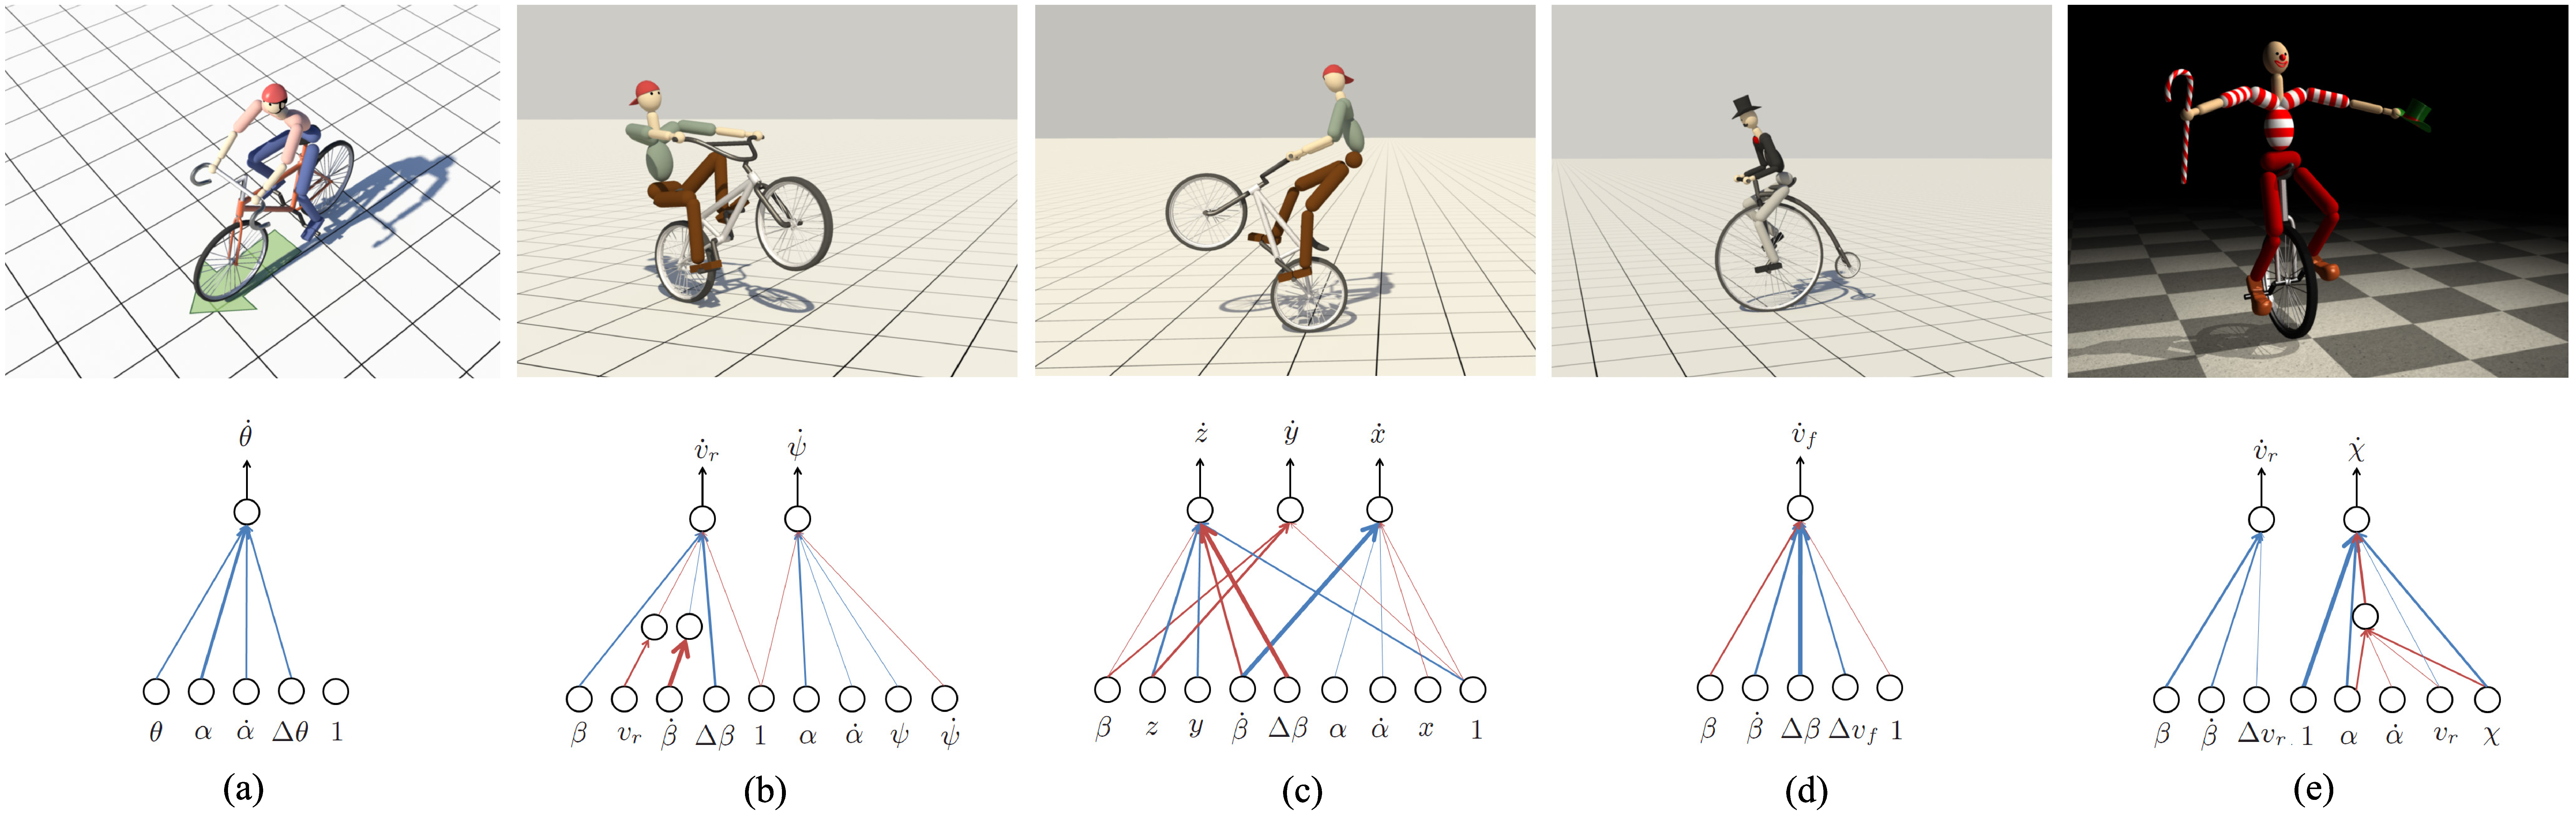
\includegraphics[width=\textwidth]{figures/bicycleNeuralNetwork.eps}
  \caption{Balance-driven tasks and the neural network structures of their corresponding controllers: (a) balance and steering, (b) wheelie, (c) back hop, (d) riding a high wheeler (stunt) and (e) riding a unicycle. Red edges have positive weights and blue edges have negative weights. The thickness of the edges shows the relative magnitudes of the weights.}
  \label{fig:neuralnet}
\end{figure}

\section{Neural Network Structures}
We used NEAT to search for both the topologies and the weights of neural networks for balance-driven tasks. In addition to the endo balance controller, which is shown in the paper, we demonstrate other learned neural networks in Figure~\ref{fig:neuralnet}. Note that NEAT performs feature selection (removing connections) for the controllers of balance and steering and back hop. It also performs structural complexification (adding nodes and connections) in the examples of the wheelie and riding a unicycle. We found that it is unintuitive to interpret these network structures, and this is a common problem of using neural networks.

\section{Reward Functions}
We summarize the reward functions that are used to learn different bicycle tasks in Table~\ref{table:rewardFunction}. We accumulate the rewards for 1000 time steps or until the bicycle loses its balance $|\alpha|>0.5$ or when the stunt fails $|\Delta \beta|>0.5$.
\begin{table}[ht]
\vspace{-0.1in}
\centering
\begin{tabular}{|l|l|}
\hline
task & reward function\\
\hline
momentum-driven & \\
\hline
going over curbs      & $\beta$ \\
endo (lifting)        & $-\beta$ \\
front wheel pivot     & $ \left\{ \begin{array}{ll} \dot{\gamma} \Delta t & \textrm{if the pivoting phase has started,}\\ 1 & \textrm{if the pivoting phase has ended,} \\ 0 & \textrm{otherwise.} \end{array} \right. $\\
bunny hop             & $h_fh_r$\\
\hline
balance-driven & \\
\hline
balance and steering  & $1 + \frac{1}{\Delta \theta+1}$ \\
wheelie               & $1 + \frac{1}{\Delta \beta + 1} + \frac{1}{\psi + 0.1} + \frac{2}{\alpha + 0.1}$ \\
endo (balance)        & $1 + \frac{1}{\Delta \beta + 1} + \frac{1}{\Delta v_f + 0.1} + \frac{1}{\alpha + 1} + \frac{1}{\theta + 1}$ \\
back hop              & $1 + \frac{1}{y + 0.1} + \frac{1}{z + 0.1} + \frac{1}{x + 0.1}$\\
high wheeler (stunt)  & $1 + \frac{1}{\Delta \beta + 1} + \frac{1}{\Delta v_f + 1} $\\
unicycle              & $1 + \frac{1}{\Delta v_r + 1} + \frac{2}{\alpha + 0.1} + \frac{1}{\chi + 1}$\\
\hline
 \end{tabular}
 \caption{Reward functions for different tasks. }
 \vspace{-0.1in}
 \label{table:rewardFunction}
 \end{table}

\section{Bicycle Specifications}
We describe the physical specifications of the three bicycles and the unicycle in Table~\ref{table:specification}.

\begin{table}[!b]
\vspace{-0.1in}
\centering
\begin{tabular}{|l|c|c|c|c|}
\hline
specification & road & BMX  & high    & uni- \\
              & bike & bike & wheeler & cycle \\
\hline
mass of the frame & 7.0 & 5.6 & 8.0 & 2.0 \\
mass of the handlebar & 3.5 & 3.5 & 4.0 & NA \\
mass of the front wheel & 1.7 & 0.71 & 5.0 & NA \\
mass of the rear wheel &  1.7 & 0.71 & 0.5 & 2.3 \\
radius of the front wheel & 0.32 & 0.25 & 0.45 & NA  \\
radius of the rear wheel & 0.32 & 0.25 & 0.11 & 0.32  \\
width of the tires & 0.015 & 0.03 & 0.015 & 0.03 \\
distance between wheels & 1.03 & 0.85 & 0.58 & NA\\
\hline
\end{tabular}
\caption{Specifications of different bicycles and the unicycle. The mass unit is $kg$ and the length unit is $m$. The distance between wheels only accounts for the horizontal distance. }
\label{table:specification}
\end{table}

\section{Simulation and Optimization Parameters}
We used Open Dynamic Engine as our physical simulator. Table~\ref{table:simParameters} summarizes the simulation parameters used in our examples.

\begin{table}[ht]
\vspace{-0.1in}
\centering
\begin{tabular}{|l|l|}
\hline
parameter & value \\
\hline
time step & 0.01s \\
constraint force mixing (CFM) & $10^{-10}$ \\
error reduction parameter (ERP) & 0.99 \\
friction coefficient (BMX bike examples) & 2.0 \\
friction coefficient (other examples) & 1.0  \\
\hline
\end{tabular}
\caption{Simulation parameters. }
\label{table:simParameters}
\end{table}

We applied CMA to search for the splines for the momentum-driven tasks. We used 90 samples per iteration, maximum of 50 iterations and the default values for other parameters \cite{Hensen:2006}.

We applied NEAT to search for the neural networks for the balance-driven tasks. The implementation can be found at Stanley \cite{Stanley:2002}. Table~\ref{table:NEATParameters} summarizes the parameters used in our NEAT optimization.

\begin{table}[ht]
\vspace{-0.1in}
\centering
\begin{tabular}{|l|l|}
\hline
parameter & value \\
\hline
max number of iterations & 50\\
population size & 90 \\
survival rate & 0.2\\
crossover rate & 0.7 \\
mutation rate & 0.2\\
chance of adding a link & 0.05\\
chance of adding a node	& 0.05\\
chance of replacing a weight & 0.1\\
max weight perturbation & 0.5\\
\hline
\end{tabular}
\caption{NEAT parameters. }
\label{table:NEATParameters}
\end{table}

